\chapter{Conclusions and outlook}
%\addcontentsline{toc}{chapter}{Conclusion and outlook} % but still display in TOC (see https://tex.stackexchange.com/a/222961)
\label{chap:conclusion}

\section{Conclusions}

In this thesis, we have laid a solid foundation for continued study of neutron stars and other kinds of compact stars.
We have derived the Tolman-Oppenheimer-Volkoff equations from general relativity, and shown how the partition function for a theory with some specified Lagrangian can be expressed as a path integral in the framework of thermal field theory.
In particular, we calculated the partition function for a cold Fermi gas composed of free Dirac neutrons and solved the Tolman-Oppenheimer-Volkoff equations with the resulting equation of state.
Finally, we applied perturbation theory to general relativity and performed a detailed analysis of stellar stability.
This work constitutes a broad and thorough introduction to the most important aspects of the study of compacts stars, starting from first principles of general relativity, quantum mechanics and field theory.

Our main results are the computed mass-radius curve in \cref{fig:nstars:massradius} and the computed stability analysis in \cref{fig:nstars:stability}.
Together, they show that neutron stars are stable up to the maximum central pressure $P_c \approx \SI{1e35}{\pascal} $ with a corresponding maximum mass $M = 0.71 \solarmass$ and minimum radius $R = \SI{9.1}{\kilo\meter}$, but become unstable for greater central pressures.
In comparison, \cite{ref:tov}, building upon the work of \cite{ref:tolman}, studied the same model in 1939 and obtained the same limit $M_\text{TOV} = 0.71 \solarmass$ with the slightly different radius $R = \SI{9.5}{\kilo\meter}$ by approximate analytical techniques.
Our computational stability analysis is also consistent with a set of qualitative rules established by \cite{ref:stability_methods} based on curvature and extrema in the mass-radius diagram.

However, most observed neutron stars exceed the mass limit we have found.
Even slowly rotating pulsars, for whom our results are comparable, \cite[section 2.1]{ref:neutron_star_physics} are typically observed with masses in the range $1.0 \solarmass < M < 2.2 \solarmass$. \cite[figure 2 and 3]{ref:neutron_star_masses_paper}
The recent observation of the gravitational wave GW170817 from the merging of two neutron stars even suggests that the true value of the upper mass limit $M_\text{TOV}$ for neutron stars, named in honor of Tolman, Oppenheimer and Volkoff, is at least $M_\text{TOV} \gtrsim 2.3 \solarmass$. \cite{ref:gravitational_wave_tov_limit}
%For ridigly rotating neutron stars, the TOV limit is believed to increase by $18\%-20\%$. \TODO{ref/drop?}

Observations of massive neutron stars give a lower bound on $M_\text{TOV}$, and hence impose constraints on stellar equations of state.
Viewed the other way around, equations of state are benchmarked by the maximum masses they produce.
Although our model performs poorly in this regard, it can in hindsight still be viewed as an interesting result because it should be close to a \emph{lower} bound on $M_\text{TOV}$.
Why?
Due to the zero-temperature approximation, \emph{all} resistance against gravitational collapse in our model is provided by the degeneracy pressure of the neutrons.
As density increases, \emph{repulsive} nuclear effects become more important and should provide \emph{additional} pressure and hence greater resistance against collapse in a real neutron star. \cite[section 3.9.8]{ref:glendenning}
Nevertheless, it is both surprising and impressive that a simple model of a neutron star as a sphere of non-interacting neutrons give estimates that are certainly of the right order of magnitude.

\section{Outlook}

From the mismatch between our results and observations, it is clear that we should seek improvements to our model.
Instead of going further in the same direction, it is also possible to turn around and pursue a different path by studying other types of stars, for example.
Let us take a look at some options available to us at the current crossroads.

\iffalse
\subsection*{Renormalization}

When we encountered infinite vacuum contributions to the energy density and pressure, we simply argued that they were unphysical and ignored them.
A more precise treatment would be to allow for additional self-interactions in the Dirac Lagrangian \eqref{eq:tft:dirac_lagrangian}, hence renormalizing the neutron mass $m$, modifying the equation of state and ultimately the mass-radius curve.
\TODO{is this correct? is the effect small?}
\TODO{is this really significant, or should i just drop it?}
%E.g. Francsco chapter 6
%Vacuum contribution diverged.
%See wikipedia intro: \url{https://en.wikipedia.org/wiki/Renormalization}
\fi

\subsection*{More advanced models with additional particles}

There is little doubt that the greatest simplification in our free Fermi gas model is that a neutron star consists \emph{only} of neutrons.
This is not true, and we should expect different results by accounting for a greater variety of particles with more advanced models.
In order to keep the model simple enough for accurate calculations, it is of practical importance to include only the particles that are most relevant.
When adding several types of charged particles, one must impose additional constraints of chemical equilibrium and charge neutrality, neither of which we have needed to worry about for the neutral neutron.
For example, \cite[chapter 4]{ref:glendenning} studies relativistic nuclear field theory and outlines a series of successive improvements to our model:

\begin{enumerate}
\begin{subequations}
\addtocounter{enumi}{-1}

\item
Our original model includes only neutrons $n$ with the free Dirac Lagrangian
\begin{equation*}
	\lagr_\psi = \bar\psi \left( i \gamma^\mu \partial_\mu - m \right) \psi 
	\qquad \big( \text{with $\hbar = c = 1$ from here on} \big) .
\label{eq:outlook:lagrangian_original}
\end{equation*}

\item
One improvement is to account for inverse beta decay $ n \rightarrow e^- + p + \bar\nu_e $ of neutrons into electrons, protons and (anti)neutrinos.
It can be shown that (anti)neutrinos will diffuse out of the star, so a simple extension is then to make the Lagrangian a sum
\begin{equation*}
	\lagr_{\psi_n} + \lagr_{\psi_p} + \lagr_{\psi_n}
\end{equation*}
of three Dirac Lagrangians of the form \eqref{eq:outlook:lagrangian_original}, with one independent field and mass corresponding to neutrons, protons and electrons.
The partition function then separates into a product of three factors, and the energy density and pressure accordingly becomes a sum of three terms of the form that we have found here.
Numerical results show that this only gives a \emph{softer} equation of state with a slightly \emph{lower} maximum mass $M_\text{TOV} = 0.70 \solarmass$, and although it is a more accurate description, it really takes us in the wrong direction. \cite[section 3.9.8]{ref:glendenning}

\item
%(Glendenning section 4.6)
Yet another improvement is made by appending the $\sigma-\omega$ model, also referred to as the Walecka model.
It consists of a scalar meson $\omega$ and a vector meson $\omega_\mu$ with
\begin{align}
	& \text{free scalar meson Lagrangian}     & \lagr_{\sigma\phantom\psi} &= \frac12 \left[ \left( \partial_\mu \sigma \right) \left( \partial^\mu \sigma \right) - m_\sigma^2 \sigma^2 \right] , \\
	& \text{free vector meson Lagrangian}     & \lagr_{\omega\phantom\psi} &= -\frac14 \omega_{\mu\nu} \omega^{\mu\nu} + \frac12 m_\omega^2 \omega_\mu \omega^\mu , \\
	& \text{scalar meson-nucleon interaction} & \lagr_{\sigma\psi} &= g_\sigma \sigma \bar\psi \psi , \\[0.5ex]
	& \text{vector meson-nucleon interaction} & \lagr_{\omega\psi} &= g_\omega \omega^\mu \bar\psi \gamma_\mu \psi , \\
	& \text{scalar self-interactions}         & \lagr_{\sigma\sigma} &= -\frac13 b m \left( g_\sigma \sigma \right)^3 - \frac14 c \left( g_\sigma \sigma \right)^4 .
\end{align}

\item
The $\sigma-\omega$ model is extended to the $\sigma-\omega-\rho$ model by including a $\rho$ meson with
\begin{align}
	& \text{free Lagrangian} & \lagr_{\rho \phantom\psi} &= -\frac14 \vec\rho_{\mu\nu} \cdot \vec\rho^{\mu\nu} + \frac12 m_\rho^2 \vec\rho_\mu \cdot \vec\rho^\mu , \\
	& \text{isospin force} & \lagr_{\rho \psi}           &= -\frac12 g_\rho \gamma_\mu \vec\rho^\mu \cdot \vec\tau \psi .
\end{align}

\item
%(Glendenning section 4.10)
Finally, the presence of neutrons, protons and electrons is generalized to that of other baryons and leptons.
Protons and neutrons are generalized to the full baryon octet
\begin{equation*}
	\left( n,\, p \right) \quad \rightarrow \quad \left( n,\, p,\, \Lambda,\, \Sigma^+,\, \Sigma^-,\, \Sigma^0,\, \Xi^-,\, \Xi^0 \right) ,
\label{eq:outlook:baryons}
\end{equation*}
while a muon is added to the lepton range
\begin{equation*}
	\left( e^- \right) \quad \rightarrow \quad \left( e^-,\, \mu^- \right) .
\label{eq:outlook:leptons}
\end{equation*}
This extension is straightforward to apply to the Lagrangians above.
For each baryon $B$, a free Dirac Lagrangian $\lagr_{\psi_B}$ and additional interaction Lagrangians with distinct couplings $g_B$ from above are added.
For each lepton $L$, only a free Dirac Lagrangian $\lagr_{\psi_L}$ is added -- their most important job is only to meet the charge neutrality constraint.
\end{subequations}
\end{enumerate}

Several fields are treated approximately in a relativistic mean field approach.
Throwing all these particles into the mix, one ends up with the quite complicated Lagrangian
\begin{equation*}
\begin{split}
	\lagr &= \sum_B \left( \lagr_{\psi_B} + \lagr_{\sigma \psi_{B}} + \lagr_{\omega \psi_{B}} + \lagr_{\rho \psi_{B}} \right) + \lagr_\sigma + \lagr_\omega + \lagr_{\sigma \sigma} + \lagr_\rho + \sum_L \lagr_{\psi_L} . \\
	      %&= \sum_B \bar\psi_B \left( i \gamma^\mu \partial_\mu - m_B + g_{\sigma B} \sigma - g_{\omega B} \gamma_\mu \omega^\mu - \frac12 g_{\rho B} \gamma_\mu \vec{\tau} \cdot \vec\rho^\mu \right) \psi_B \\
	      %&+ \frac12 \left[ \left( \partial_\mu \sigma \right)^2 - m_\sigma^2 \sigma^2 \right] - \frac14 \omega_{\mu \nu}^2 + \frac12 m_\omega^2 \omega_\mu^2 \\
	      %&- \frac14 \vec\rho_{\mu\nu}^2 + \frac12 m_\rho^2 \vec\rho_\mu^2 - \frac13 b m_n \left( g_\sigma \sigma \right)^3 - \frac14 c \left( g_\sigma \sigma \right)^4 \\
	      %&+ \sum_L \bar\psi_L \left( i \gamma^\mu \partial_\mu - m_L \right) \psi_L ,
\end{split}
\end{equation*}
With all these effects, numerical results give a maximum mass in the range $1.42 \solarmass < M_\text{TOV} < 2.02 \solarmass$ depending on the values chosen for the coupling constants. \cite[table 1]{ref:neutron_star_hyperon_effect}
This is much more in line with observations.
For a gradual, step-by-step exposure to these successive improvements, see also the theses \cite{ref:master_caroline,ref:master_francesco}.

\subsection*{Rotating neutron stars}

Since observed neutron stars are pulsars, another relevant path of study is that of rotating neutron stars.
A rotating neutron star breaks spherical symmetry, but retains axial symmetry about its rotation axis.
This requires a more advanced treatment of general relativity, where the spherically symmetric metric \eqref{eq:tov:metric} must be replaced with the axially symmetric metric
\cite[section 6]{ref:glendenning}
\begin{equation*}
	%\dif s^2 = e^{2 \nu} \dif t^2 - e^{2 \psi} \left( \dif r^2 + r^2 \dif \theta^2 \right) - e^{2 \psi} \left( \dif \phi - \omega \dif t \right)^2
	\dif s^2 = e^{2\nu(r,\theta)} c^2 \dif t^2 - e^{2\lambda(r,\theta)} \dif r^2 - r^2 e^{2 \mu(r,\theta)} \left\{ \dif \theta^2 + \sin^2 \theta \left[ \dif \theta  - \omega(r,\theta) \dif t \right]^2 \right\} ,
\end{equation*}
and the fluid's four-velocity $u^\mu = (u^0, 0, 0, u^3)$ gains an angular component $u^3 = \odv{\phi}/{\tau}$ in equilibrium.
The star is then no longer governed by the familiar Tolman-Oppenheimer-Volkoff equations, which were derived under the assumption of no rotation.
Study of rotating neutron stars is useful because it is directly comparable to observations of pulsars.

\iffalse
\subsubsection{Charge neutrality}

% See e.g. Glendenning page 71, Halvor 
Multiple particles may in general have charge, in contrast to neutrons.
Stars are neutral: if it is charged, then particles of the same signed charge as the star are kicked out due to strong Coulomb force relative to weak gravitational force (can show quantitatively).
This argument means \emph{global} charge neutrality, but it is more common, easier and has little effect to instead assume \emph{local} charge neutrality.
\fi

\iffalse
\subsection*{Exotic stars}

Another possible path of pursuit is to go looking for different types of stars.
It is speculated that neutron stars that only slightly exceed the Tolman-Oppenheimer-Volkoff limit need not necessarily collapse to black holes, but can form other hypothetical, compact stars referred to as \emph{exotic stars}.
Observations have identified several candidates for exotic stars with masses in the gap between the upper Tolman-Oppenheimer-Volkoff limit and the least massive observed black holes, but of unknown nature. \cite{ref:wiki_list_star_massess}
For example, it is possible that a neutron star that exceeds the limit can evolve into a \emph{quark star}, where individual neutrons no longer play the most important role, but their constituent quarks have broken free and become \emph{deconfined quark matter}.
This state of matter is only stable under extreme temperature and pressure, and it is also possible that it exists in the core of ordinary neutron stars. \cite[chapter 8]{ref:glendenning}
Other examples of exotic stars are strange stars, electroweak stars, preon stars and boson stars.

\subsection*{Hybrid stars}

Another unrealistic assumption in this and even more advanced neutron star models is that the same type of matter is distributed throughout the neutron star -- all the way from the core to the very surface.
In a real star, it is natural to expect a phase transition somewhere between the surface and the core.
The term \emph{hybrid stars} refers to stars with mixed-phase interiors. \cite[chapter 9]{ref:glendenning}
To come closer to an answer regarding what lies in the core of a neutron star, one must dare to study such stars and models.
\fi

\subsection*{Hybrid stars and quark stars}

\begin{figure}
\centering
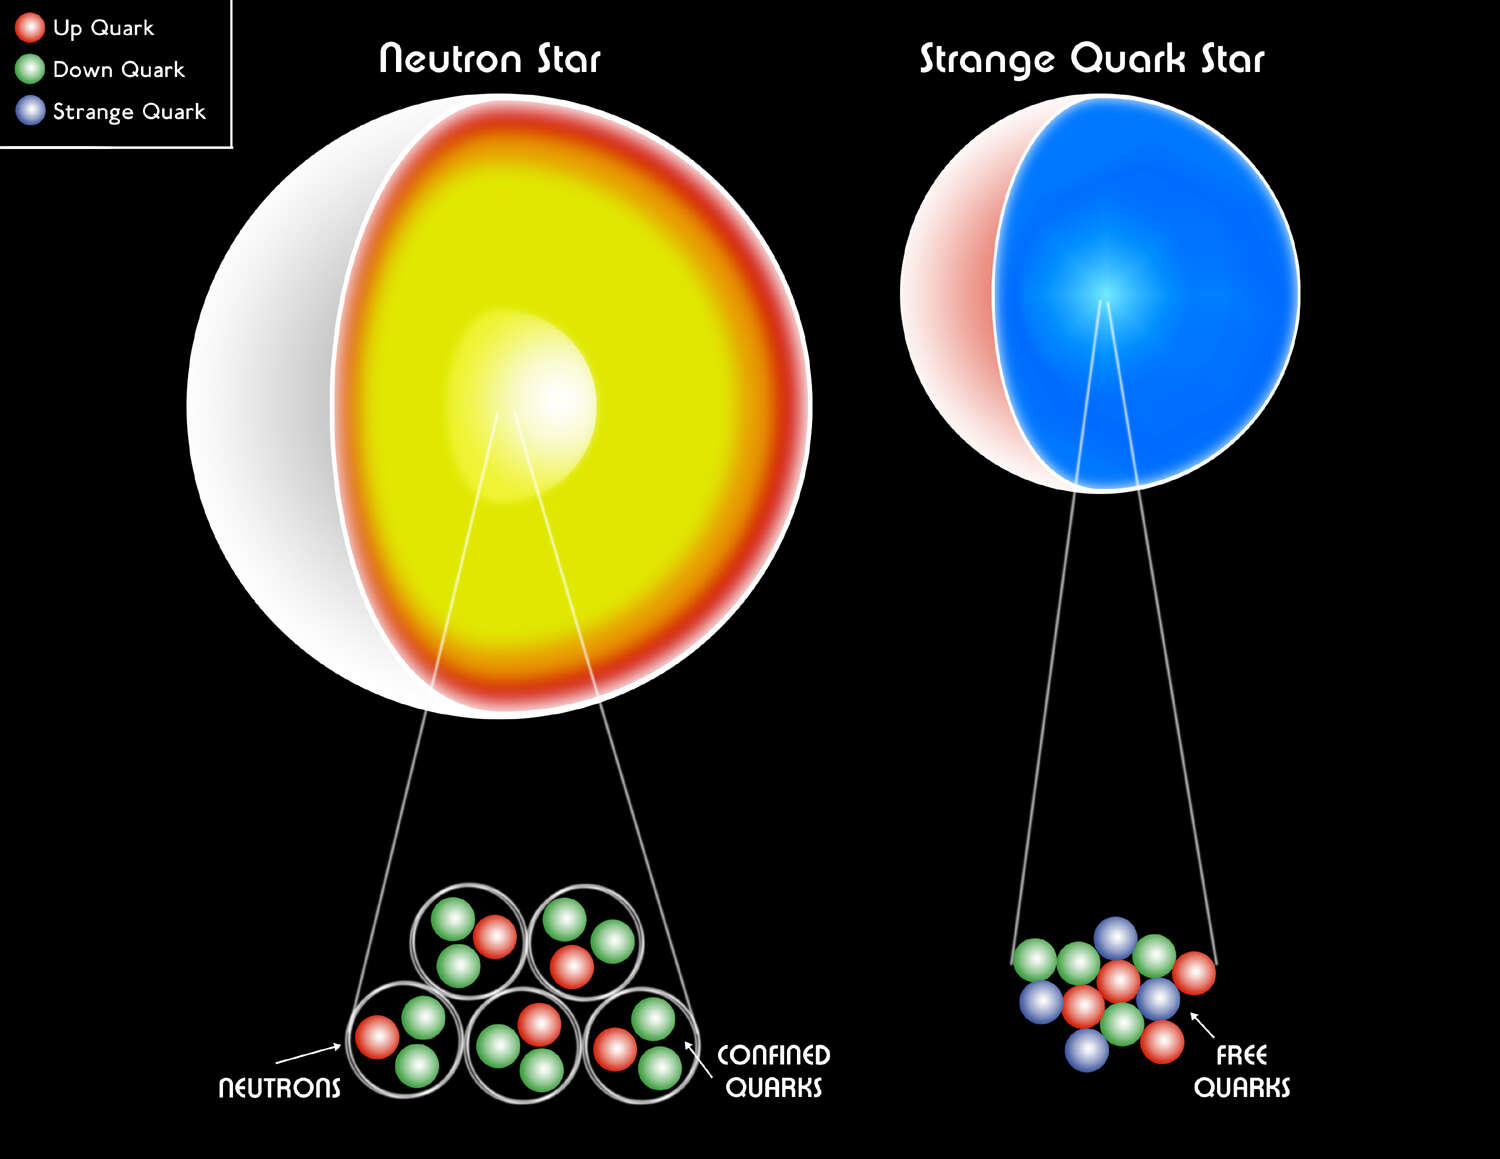
\includegraphics[width=0.6\textwidth]{figures/neutron-quark-star-optimized.jpg}
\caption{\label{fig:conclusion:neutron_vs_quark_star}%
	In a neutron star, quarks are confined in neutrons.
	In a hypothetical quark star, the density is so extreme that quarks are deconfined from neutrons.
	\credit{Chandra X-ray Observatory / M. Weiss}{https://chandra.harvard.edu/photo/2002/0211/more.html}
}
\end{figure}

Neutrons are composed of quarks, and quarks are described by quantum chromodynamics.
This theory features \emph{asymptotic freedom}.
At extreme density, it causes quarks to become free of interactions, resulting in a new state of matter known as \emph{quark matter}.
As illustrated in \cref{fig:conclusion:neutron_vs_quark_star}, neutrons lose their individuality, and it is instead free quarks that make up the fundamental degrees of freedom.
%In fact, it is likely that the universe passed through a phase of quark matter during the first few seconds.
It is speculated that the conditions in the cores of neutron stars are so extreme that it allows for the presence of quark matter.
If this is true, some or all neutron stars may really be \emph{hybrid stars} with a phase transition between a central quark matter core surrounded by a nuclear matter envelope.
\emph{Quark stars} refer to such hypothetical stars composed of pure quark matter only, with no nuclear envelope.
\cite[chapter 8]{ref:glendenning}

Indeed, there have been observed objects of unknown nature whose mass exceeds the currently accepted value of Tolman-Oppenheimer-Volkoff limit, but falls short of the least massive known black holes. \cite{ref:wiki_list_star_massess}
These objects may turn out to be neutron stars or black holes after all, but they are also candidates for hybrid stars and quark stars -- both of which are hypothetical objects yet to be observed.

Unfortunately, it is notoriously difficult to make practical computations of quantum chromodynamics.
Therefore, alternative and more practical models such as the \emph{MIT bag model} have been developed to study quark stars.

It is this path that I aim to study in my master thesis following this specialization project.

%\subsection*{Bottom line}
%We have only scratched the surface of neutron stars.
%At the core, there are still a great deal of unanswered questions that we can pursue.
